\begin{todolist}
    \item what is histamine, why we want to detect it
    \item histamine aptamers
    \item CV
    \item EIS
    \item transfer curves
    \item current vs time
\end{todolist}

\note{To achieve selective detection of histamine using an electrolyte-gated field-effect transistor (EG-FET), the functionalization of the gate electrode is essential. Without a dedicated sensing layer, the device lacks specificity and may respond to various interfering species. This section describes the modification of the gate with a histamine-selective recognition element, enabling precise and reliable detection.}

\begin{figure}
    \centering
    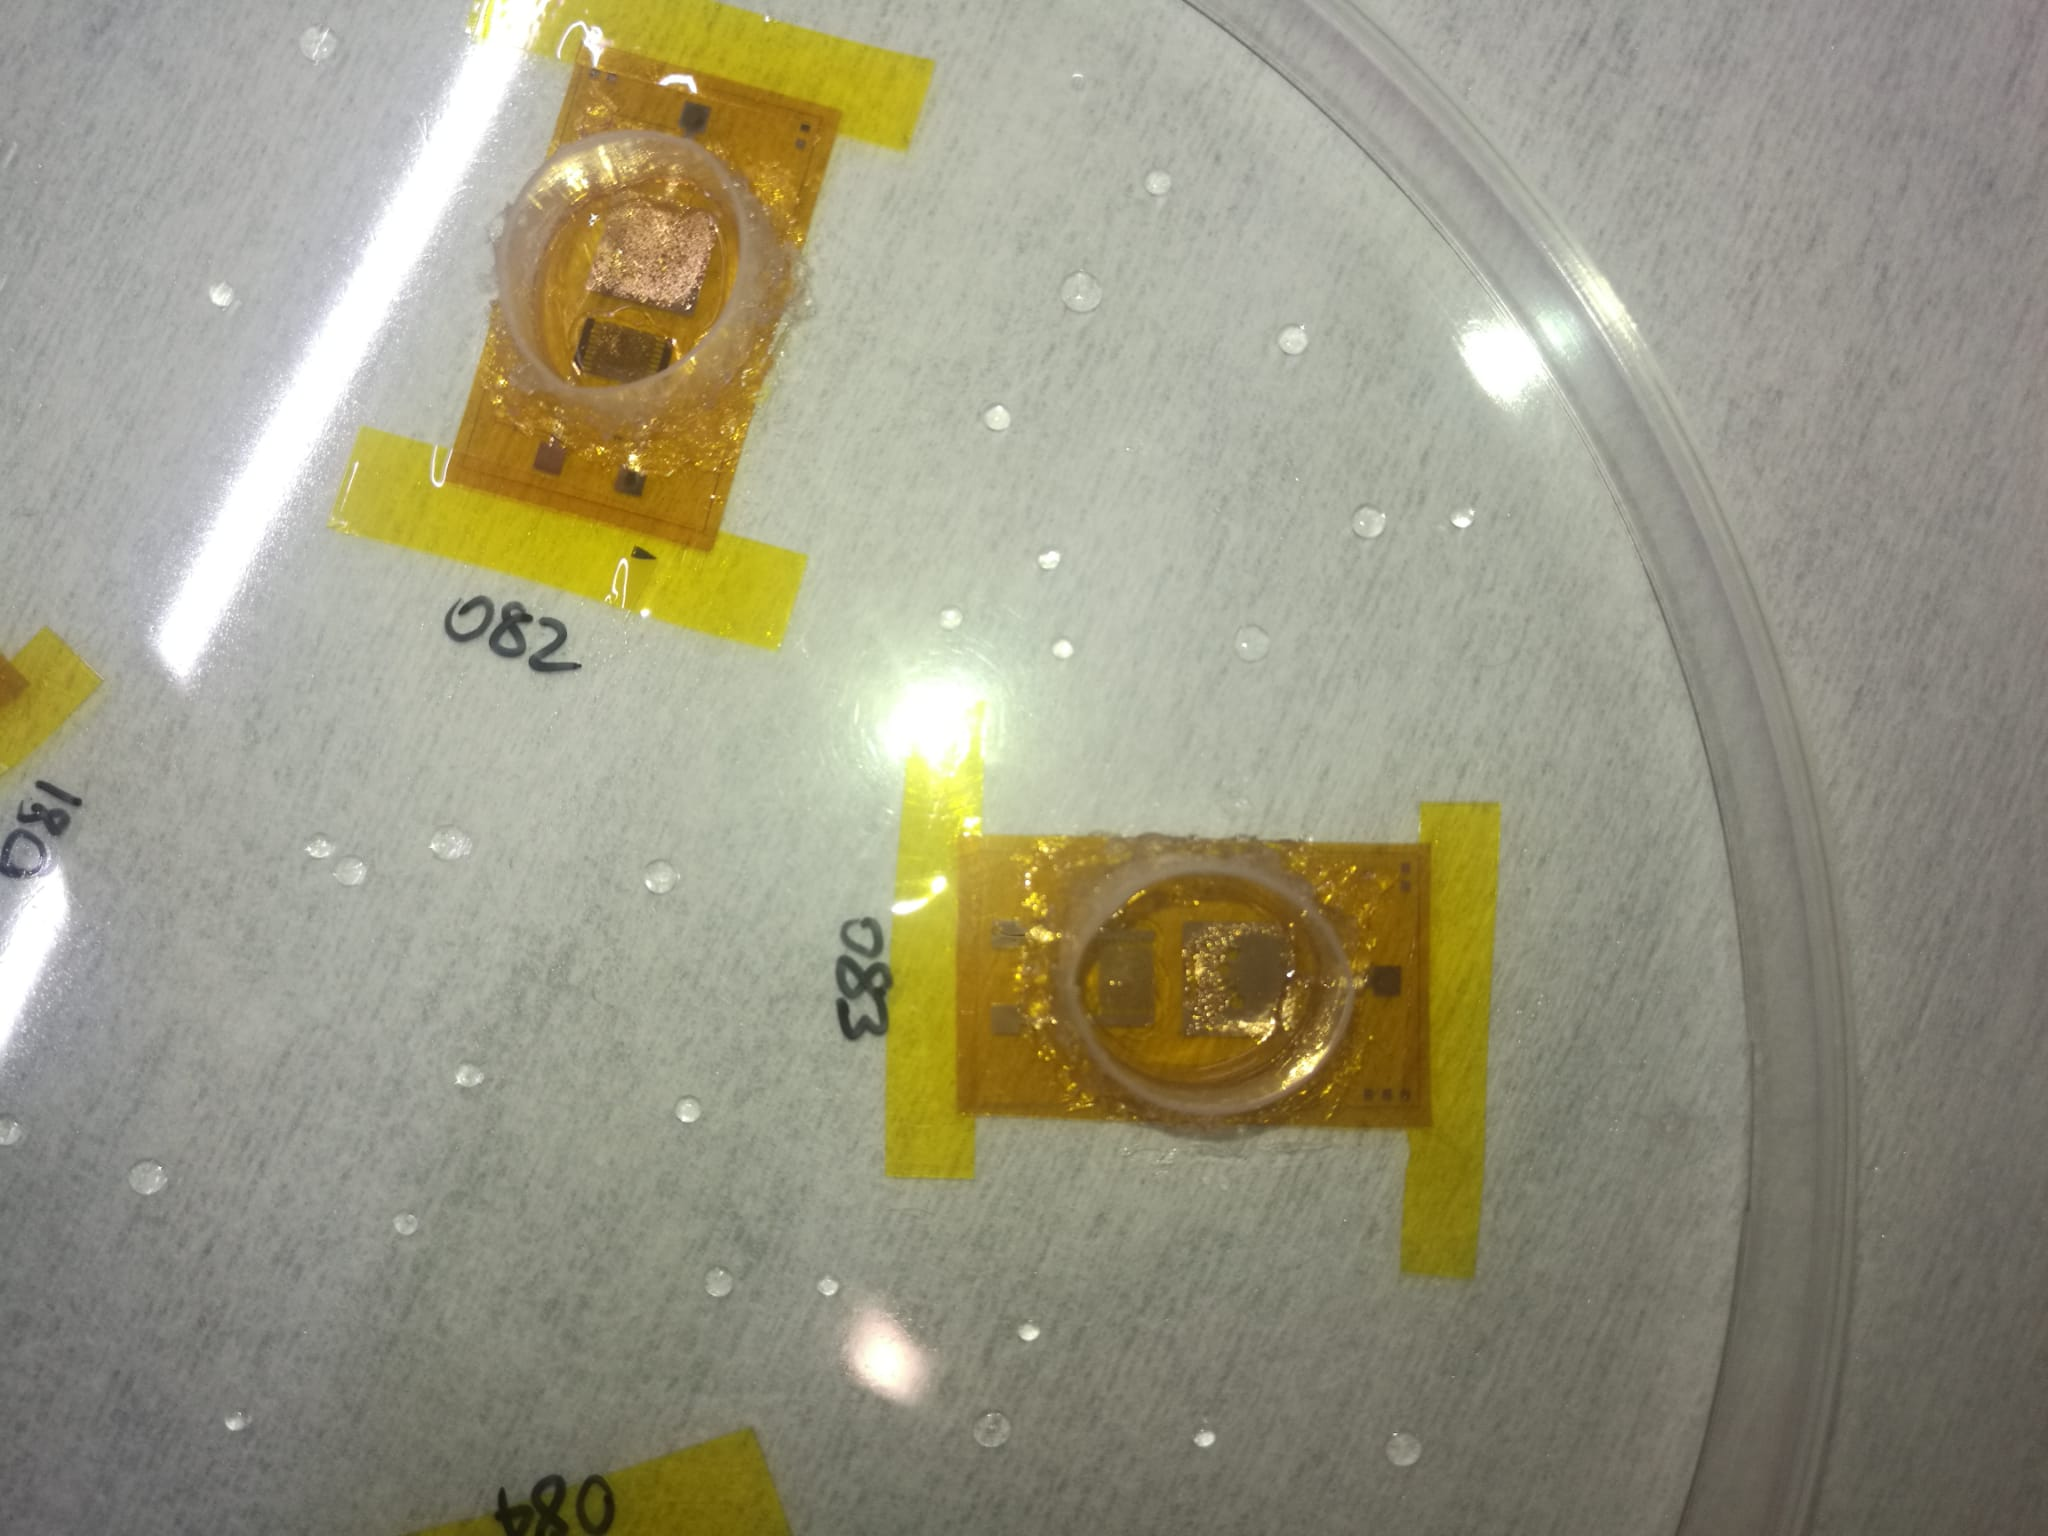
\includegraphics[width = 0.4\textwidth]{figures/chapter4/histamine/cleaningDamages.jpeg}
    \caption{}
    \label{fig:cleaningDamages}
\end{figure}

\begin{figure}
    \centering
    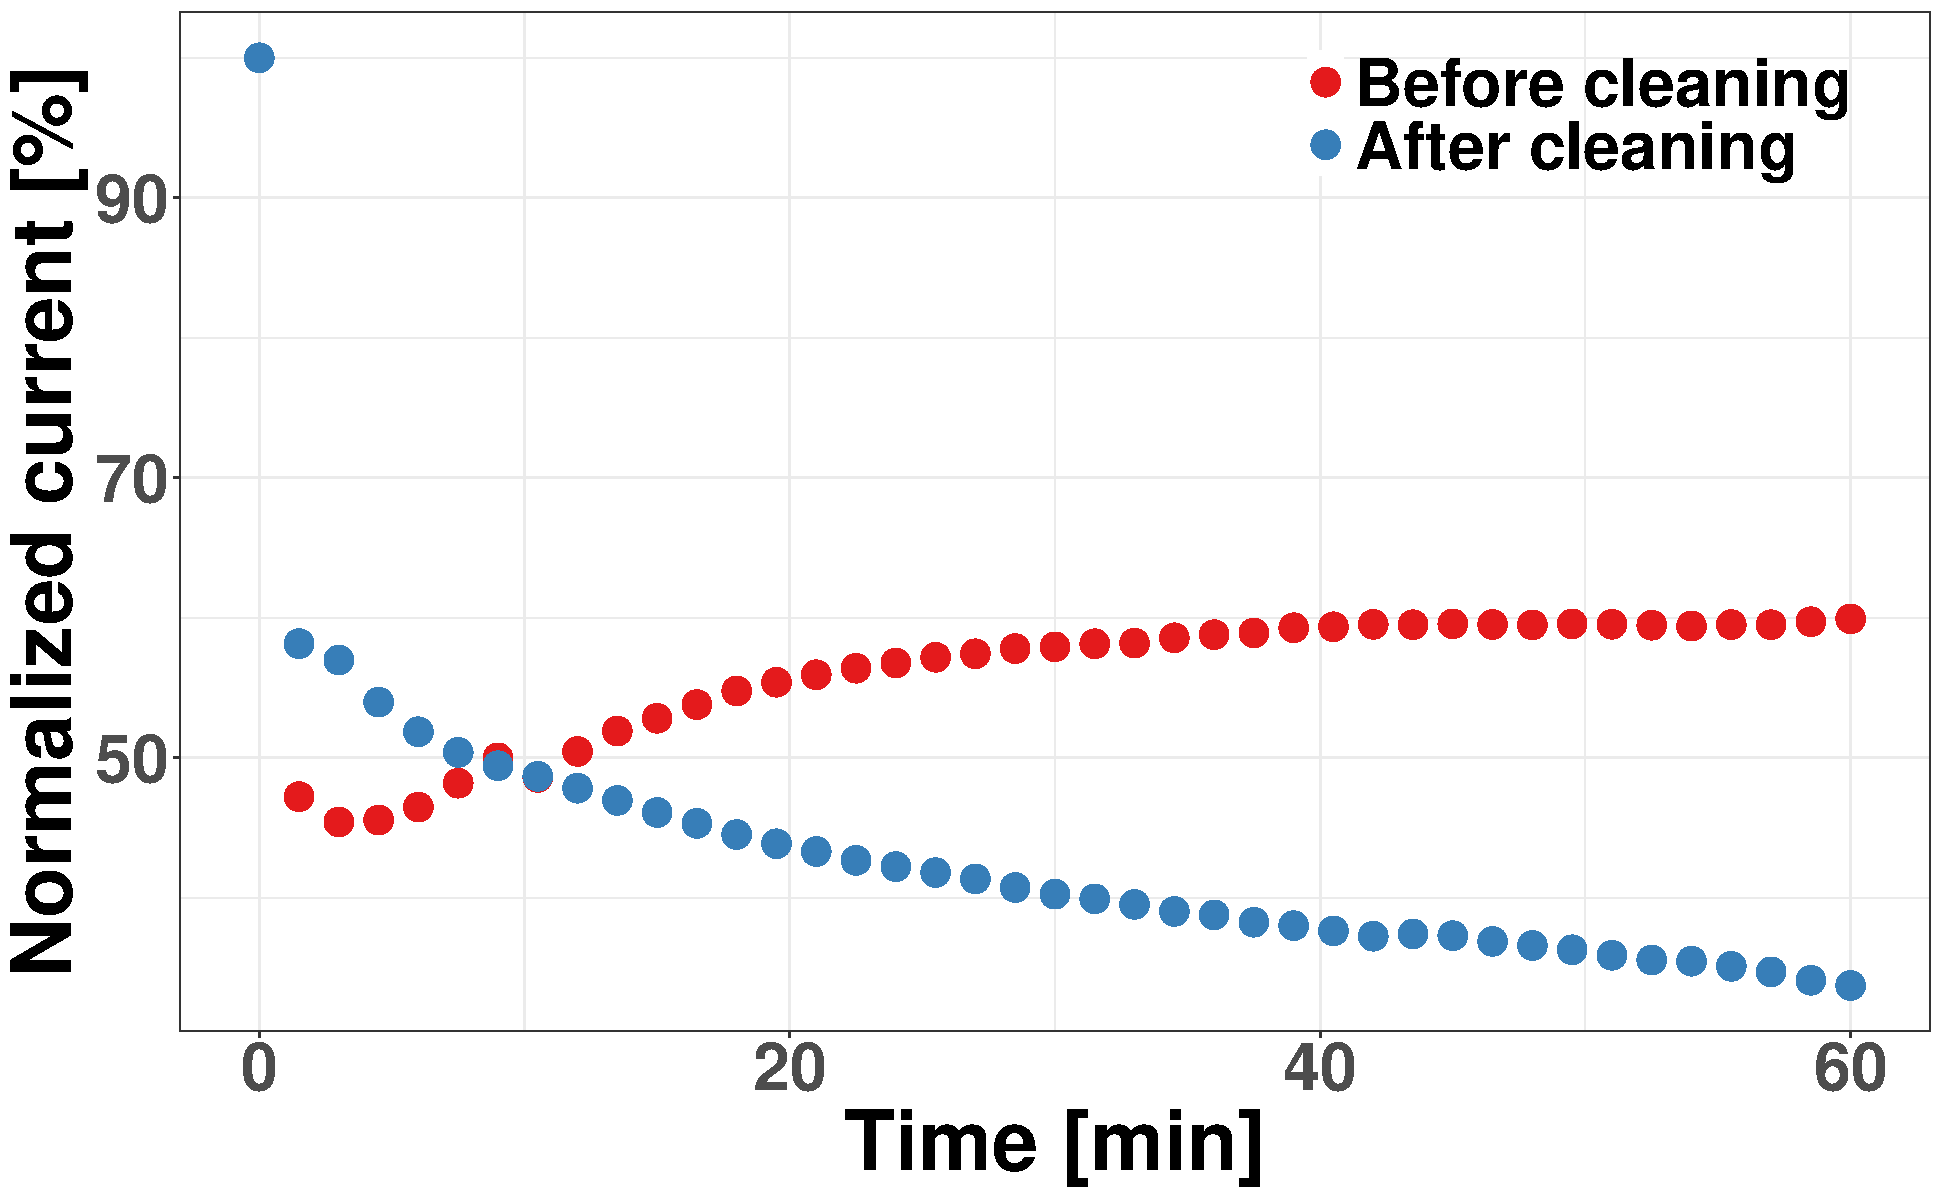
\includegraphics[width = 0.4\textwidth]{figures/chapter4/histamine/BeforeAfterClean.pdf}
    \caption{}
    \label{fig:BeforeAfterClean}
\end{figure}

\begin{figure}
    \centering
    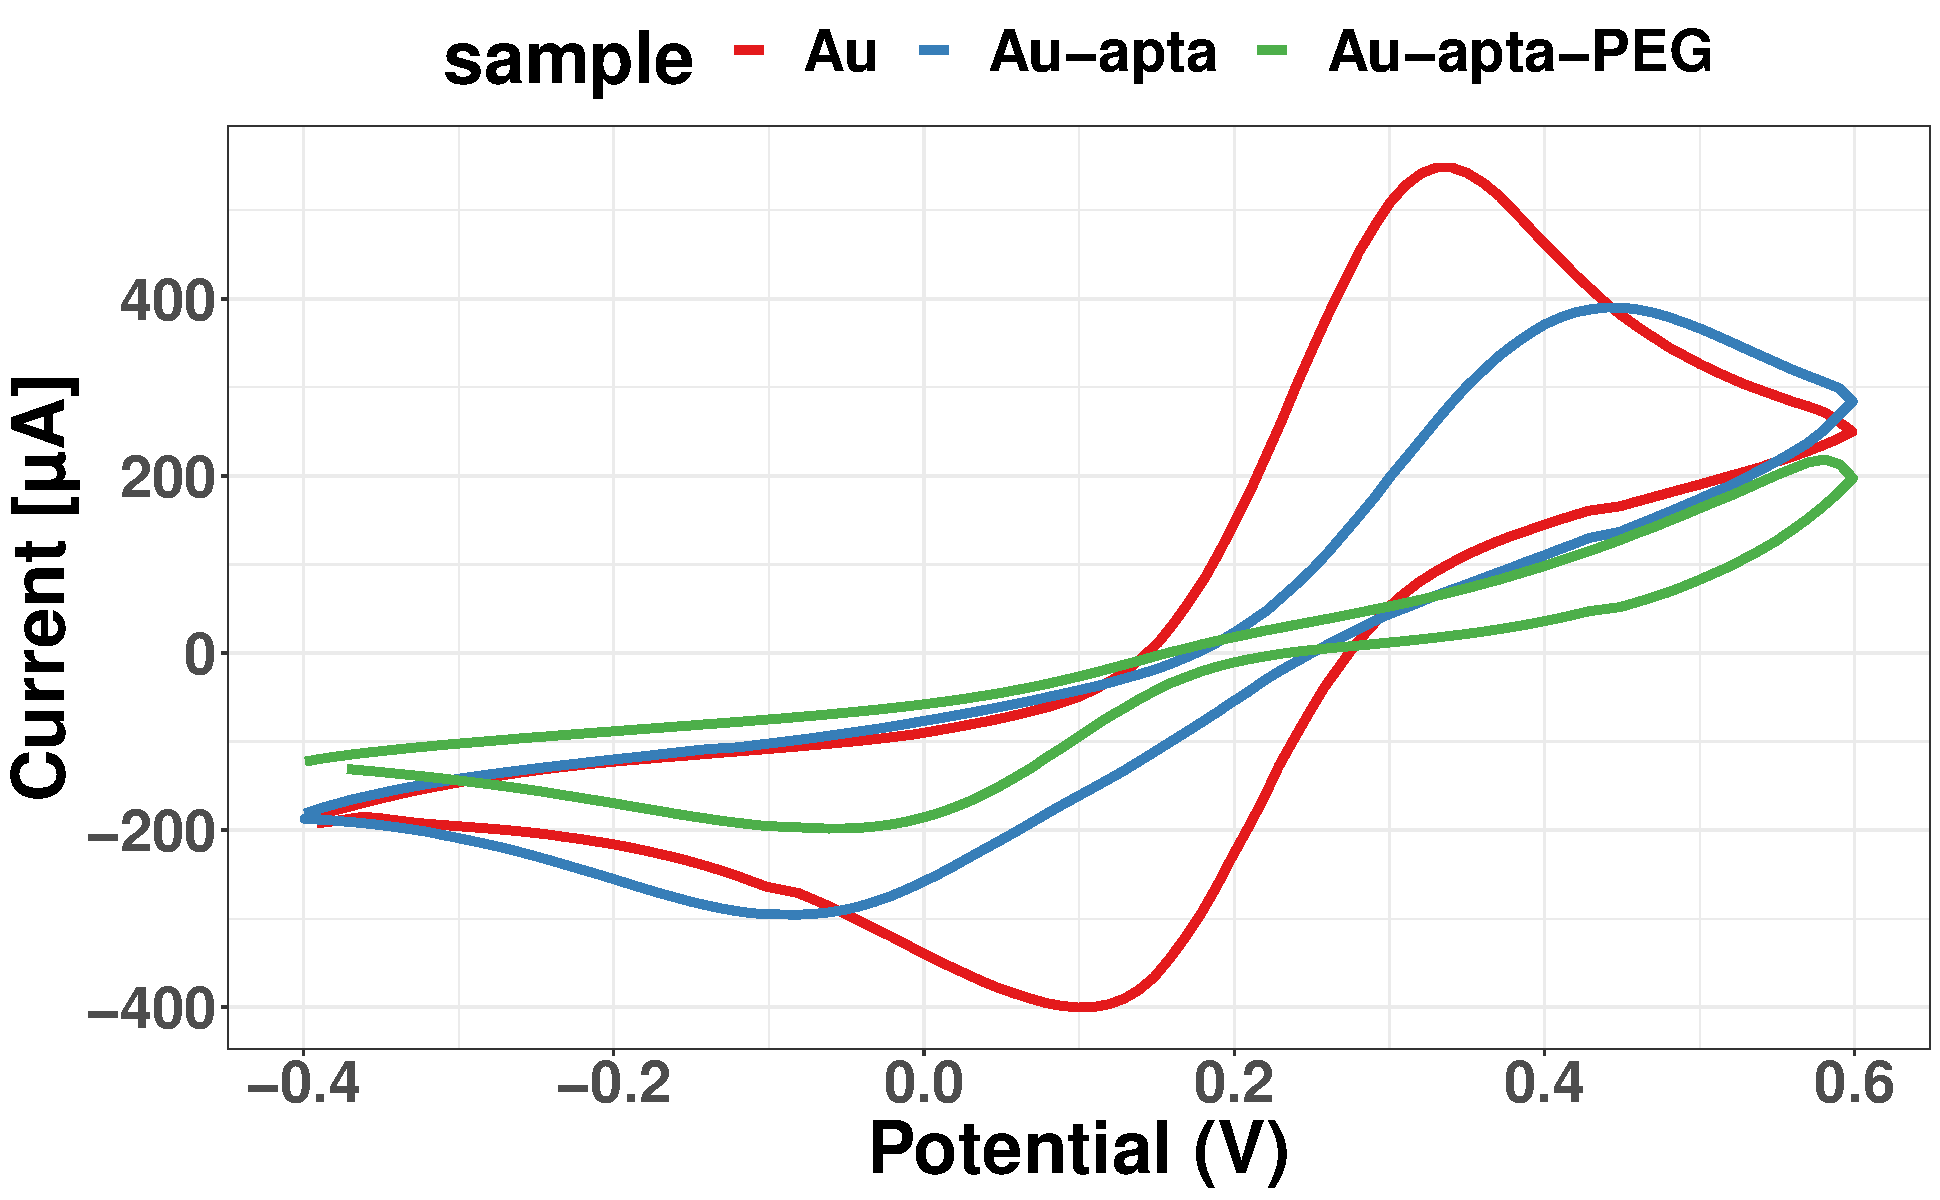
\includegraphics[width = 0.4\textwidth]{figures/chapter4/histamine/CV_functionalization.pdf}
    \quad
    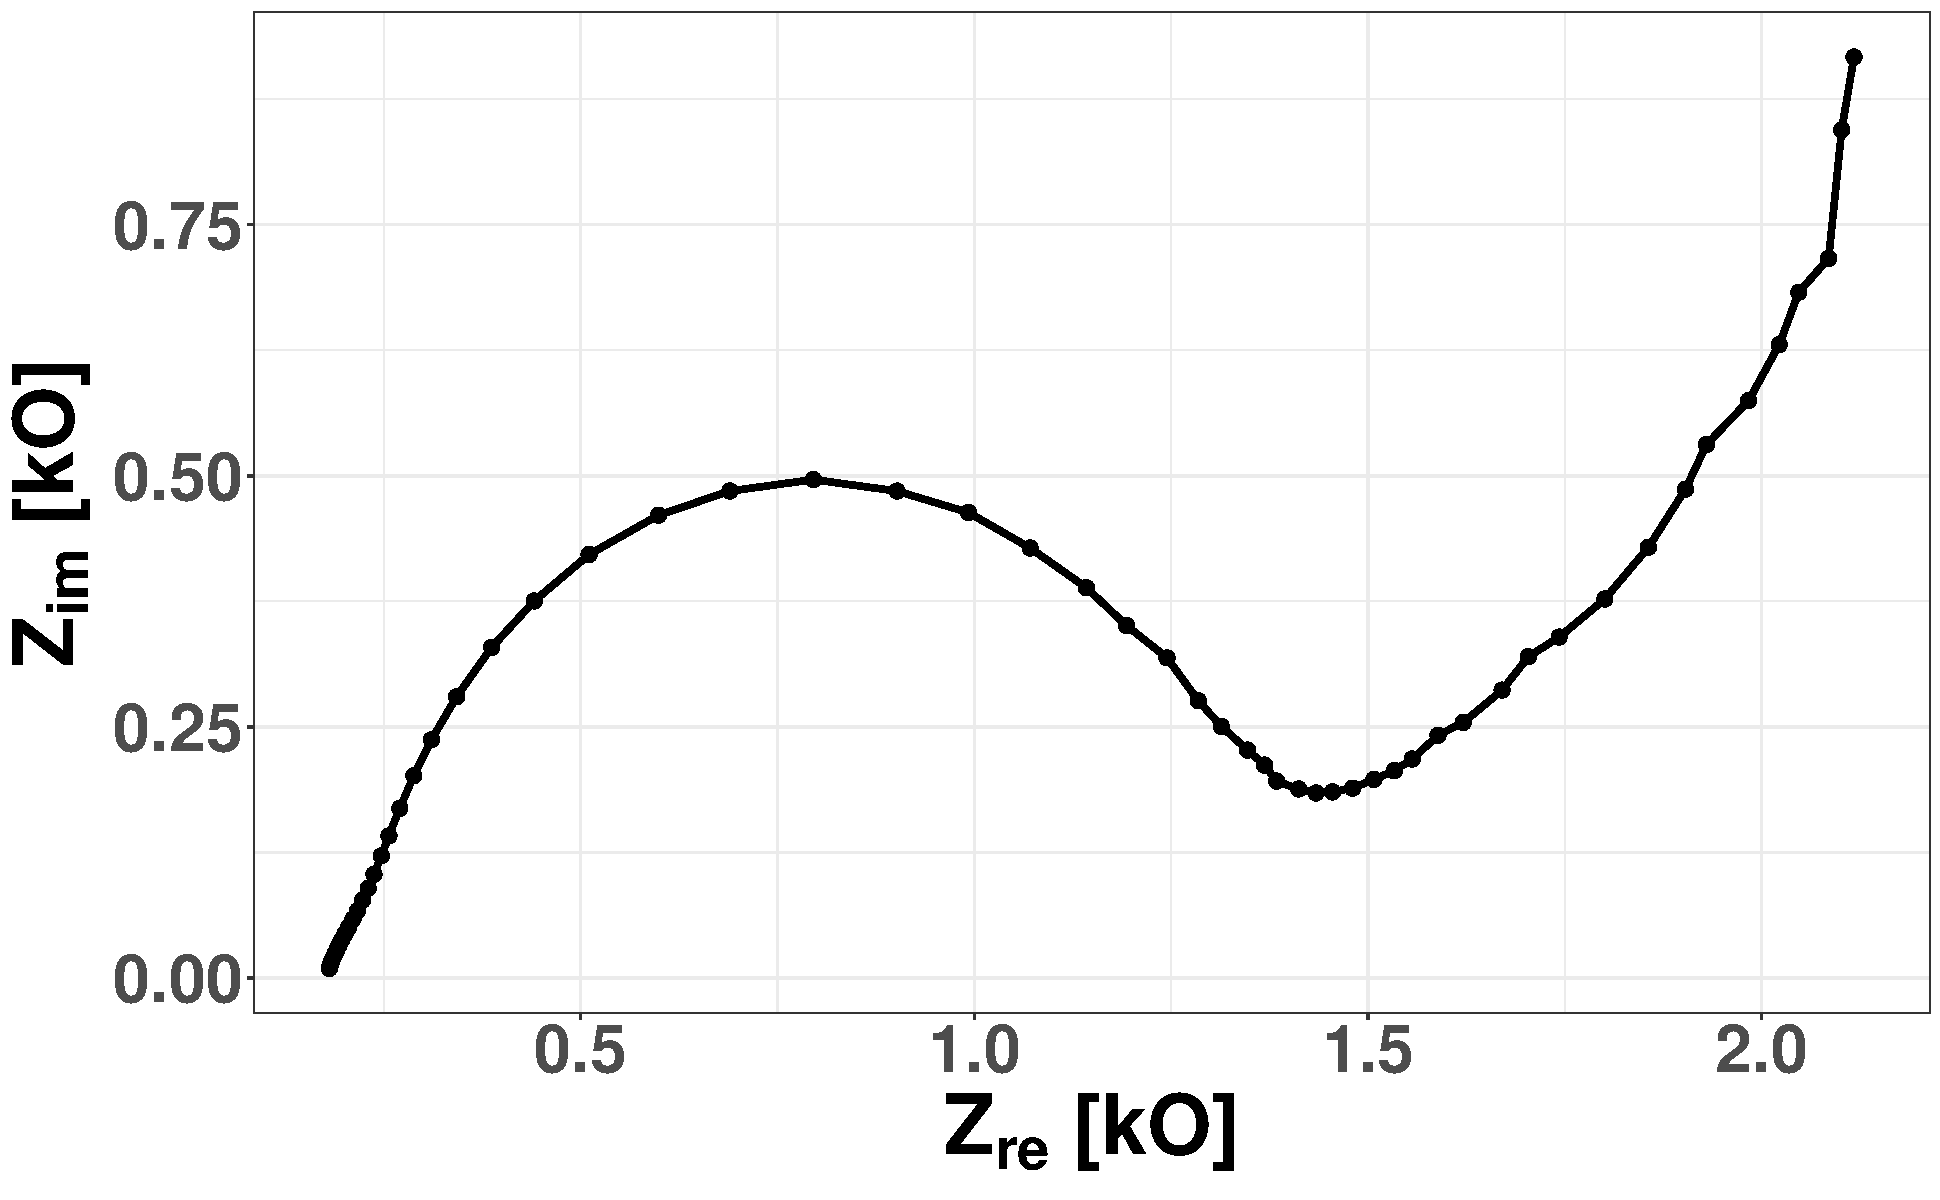
\includegraphics[width = 0.4\textwidth]{figures/chapter4/histamine/EIS_functionalization_gold.pdf}
    \caption{}
    \label{fig:CVfunctionalization}
\end{figure}

\begin{figure}
    \centering
    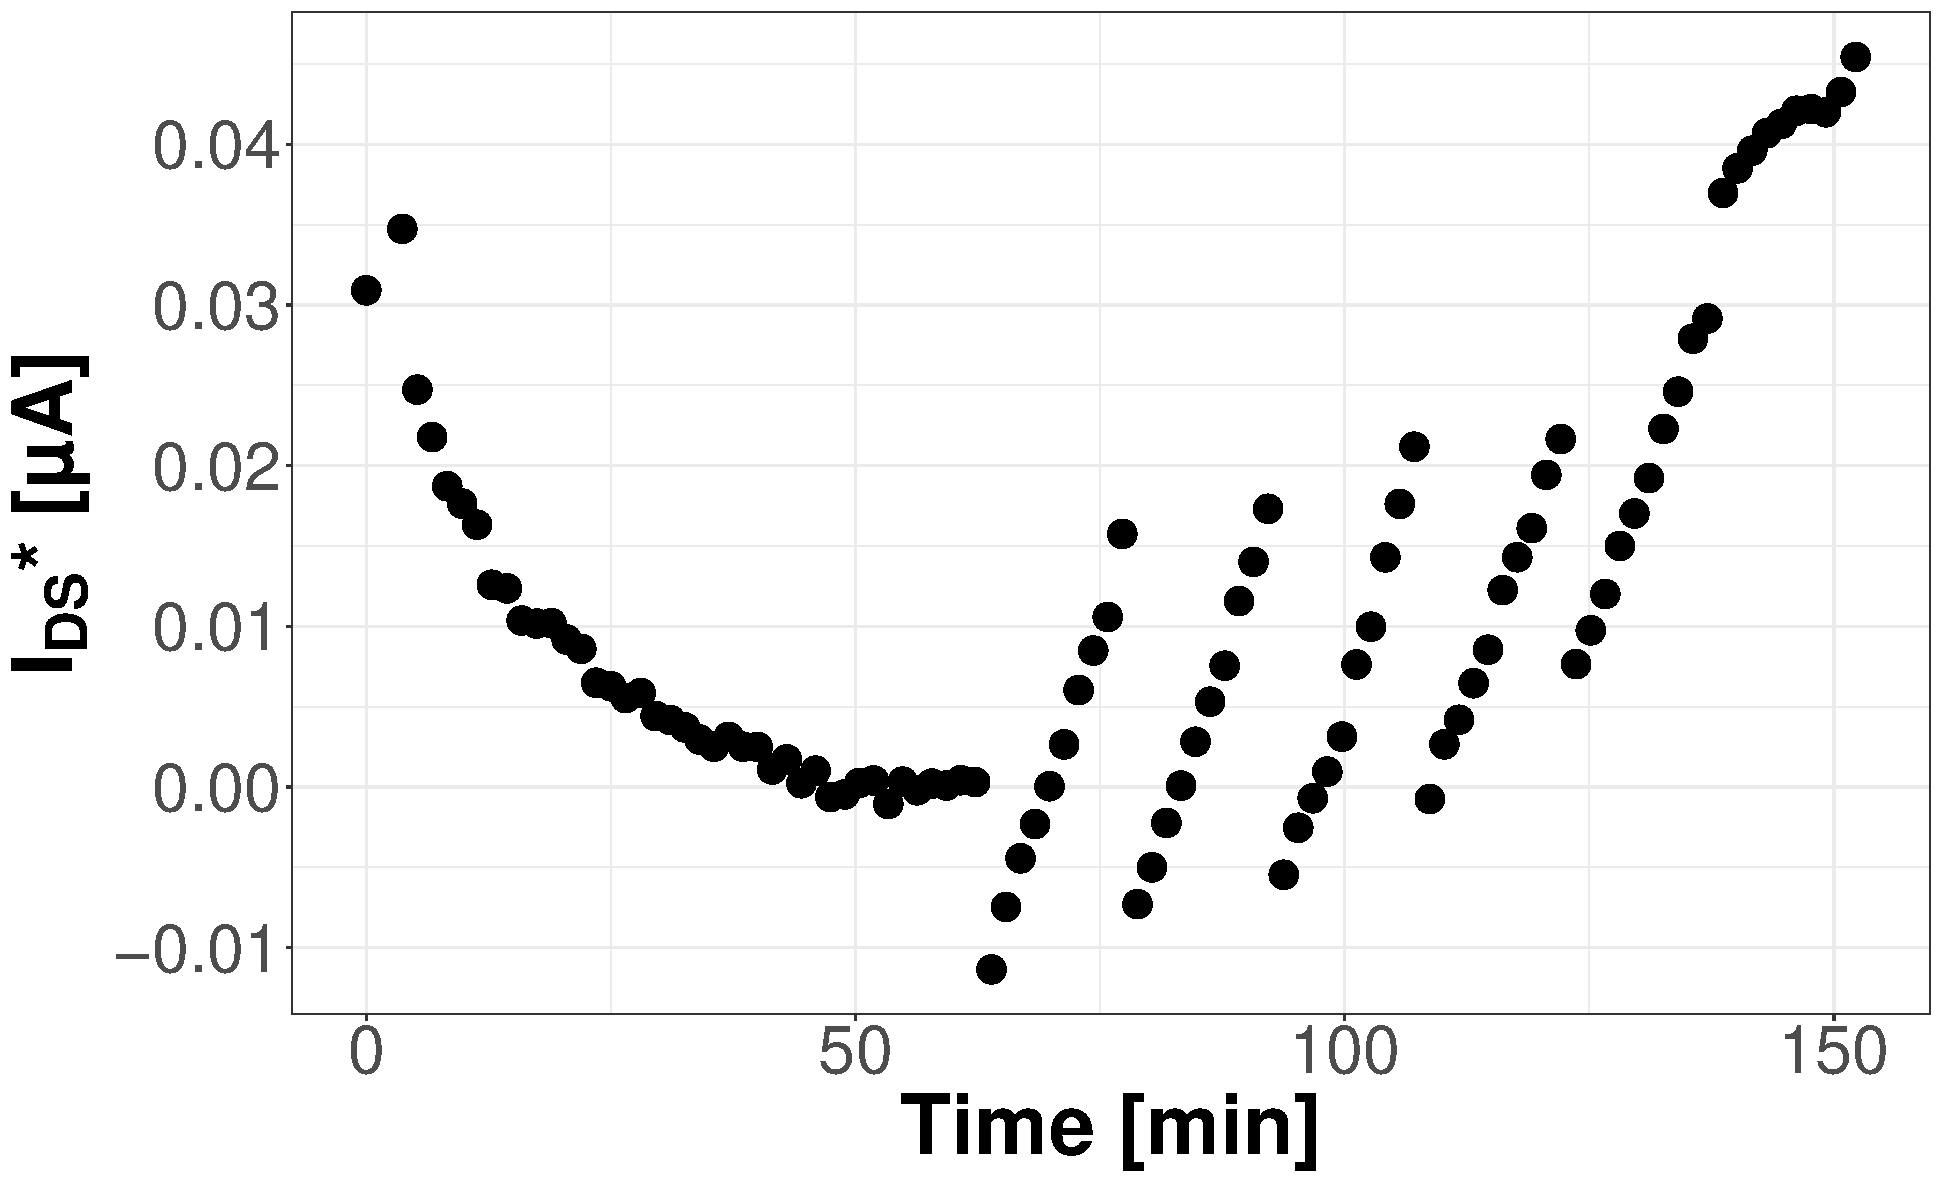
\includegraphics[width = 0.4\textwidth]{figures/chapter4/histamine/correctedPlot-transfers.pdf}
    \quad
    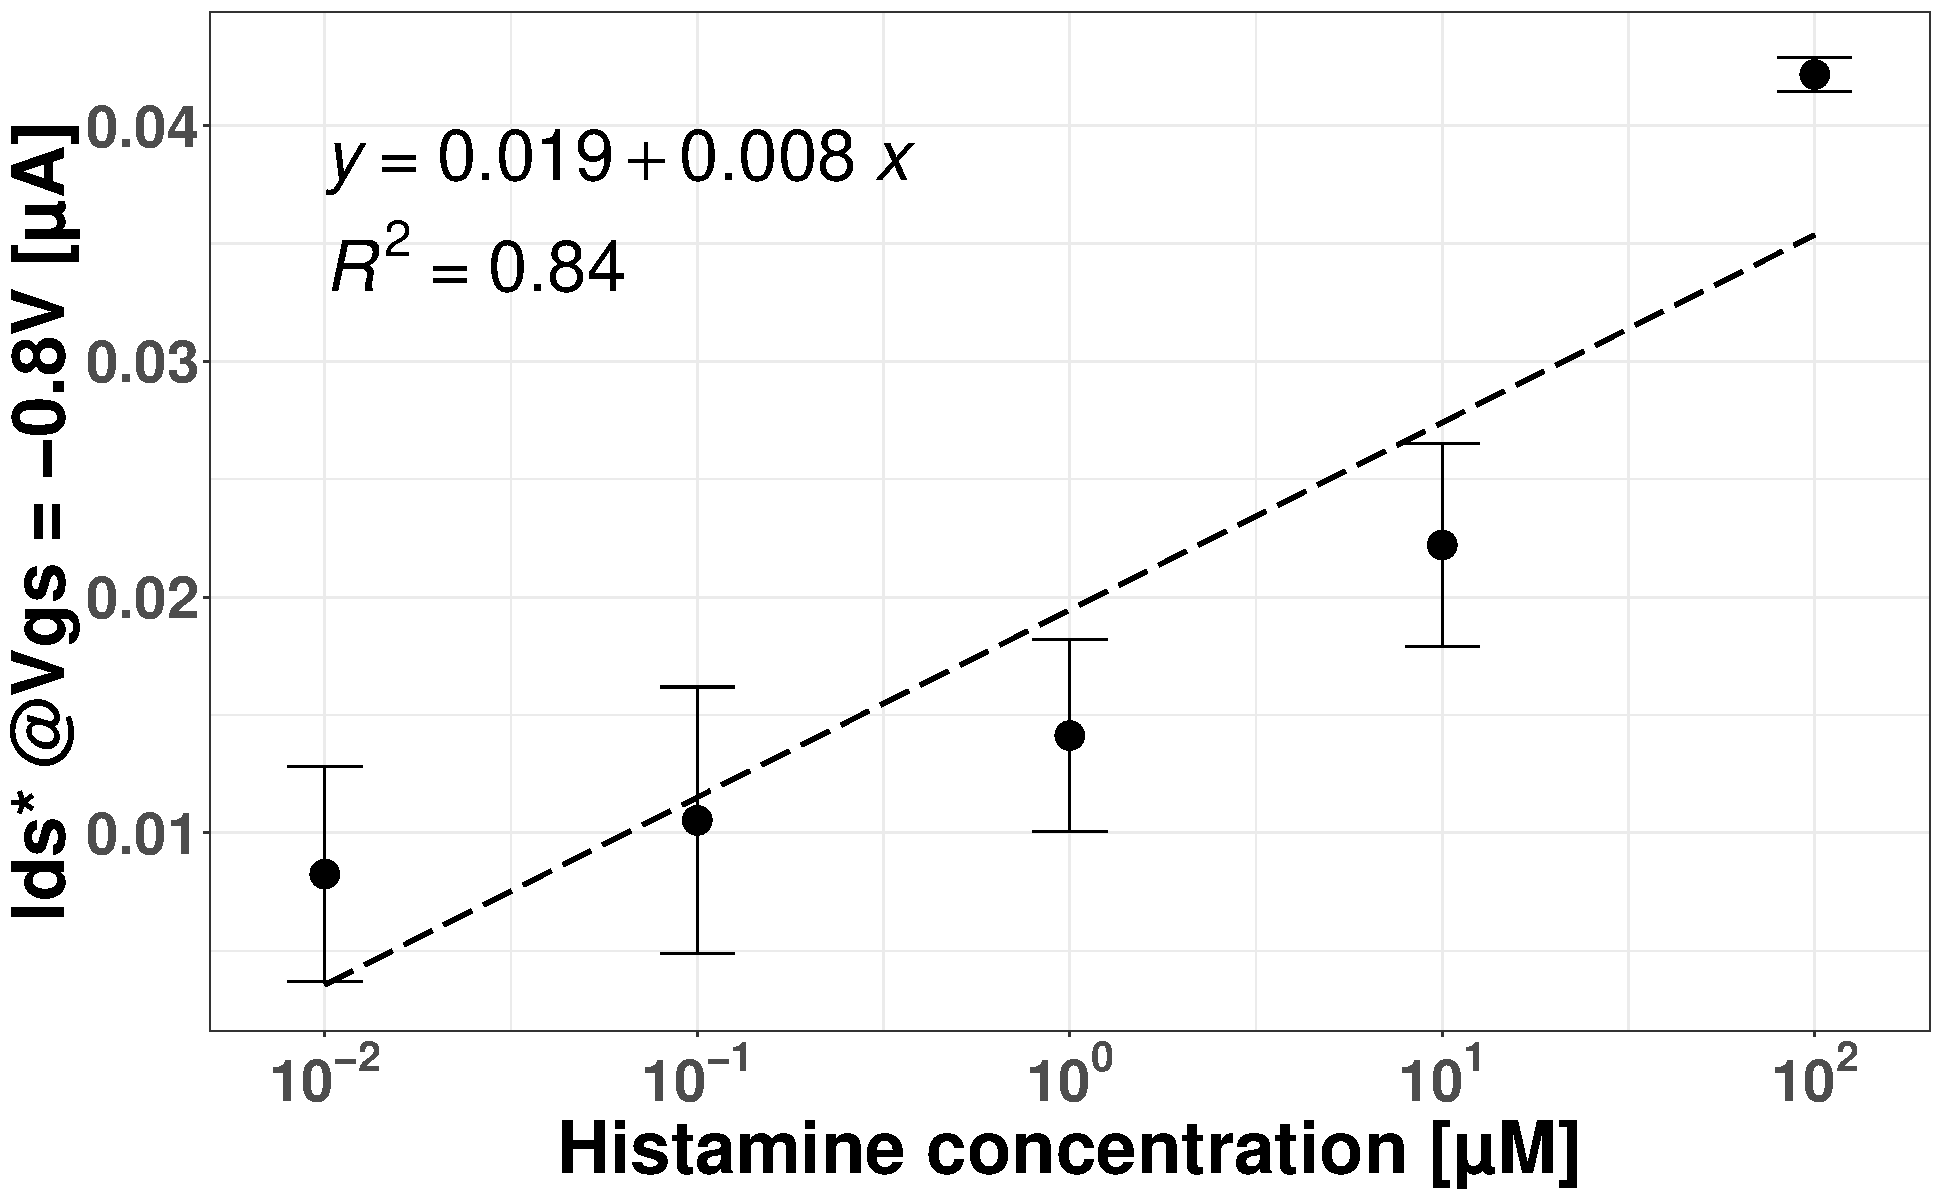
\includegraphics[width = 0.4\textwidth]{figures/chapter4/histamine/calibrationPlot-transfers.pdf}
    \caption{}
    \label{fig:HisTransfers}
\end{figure}

\begin{figure}
    \centering
    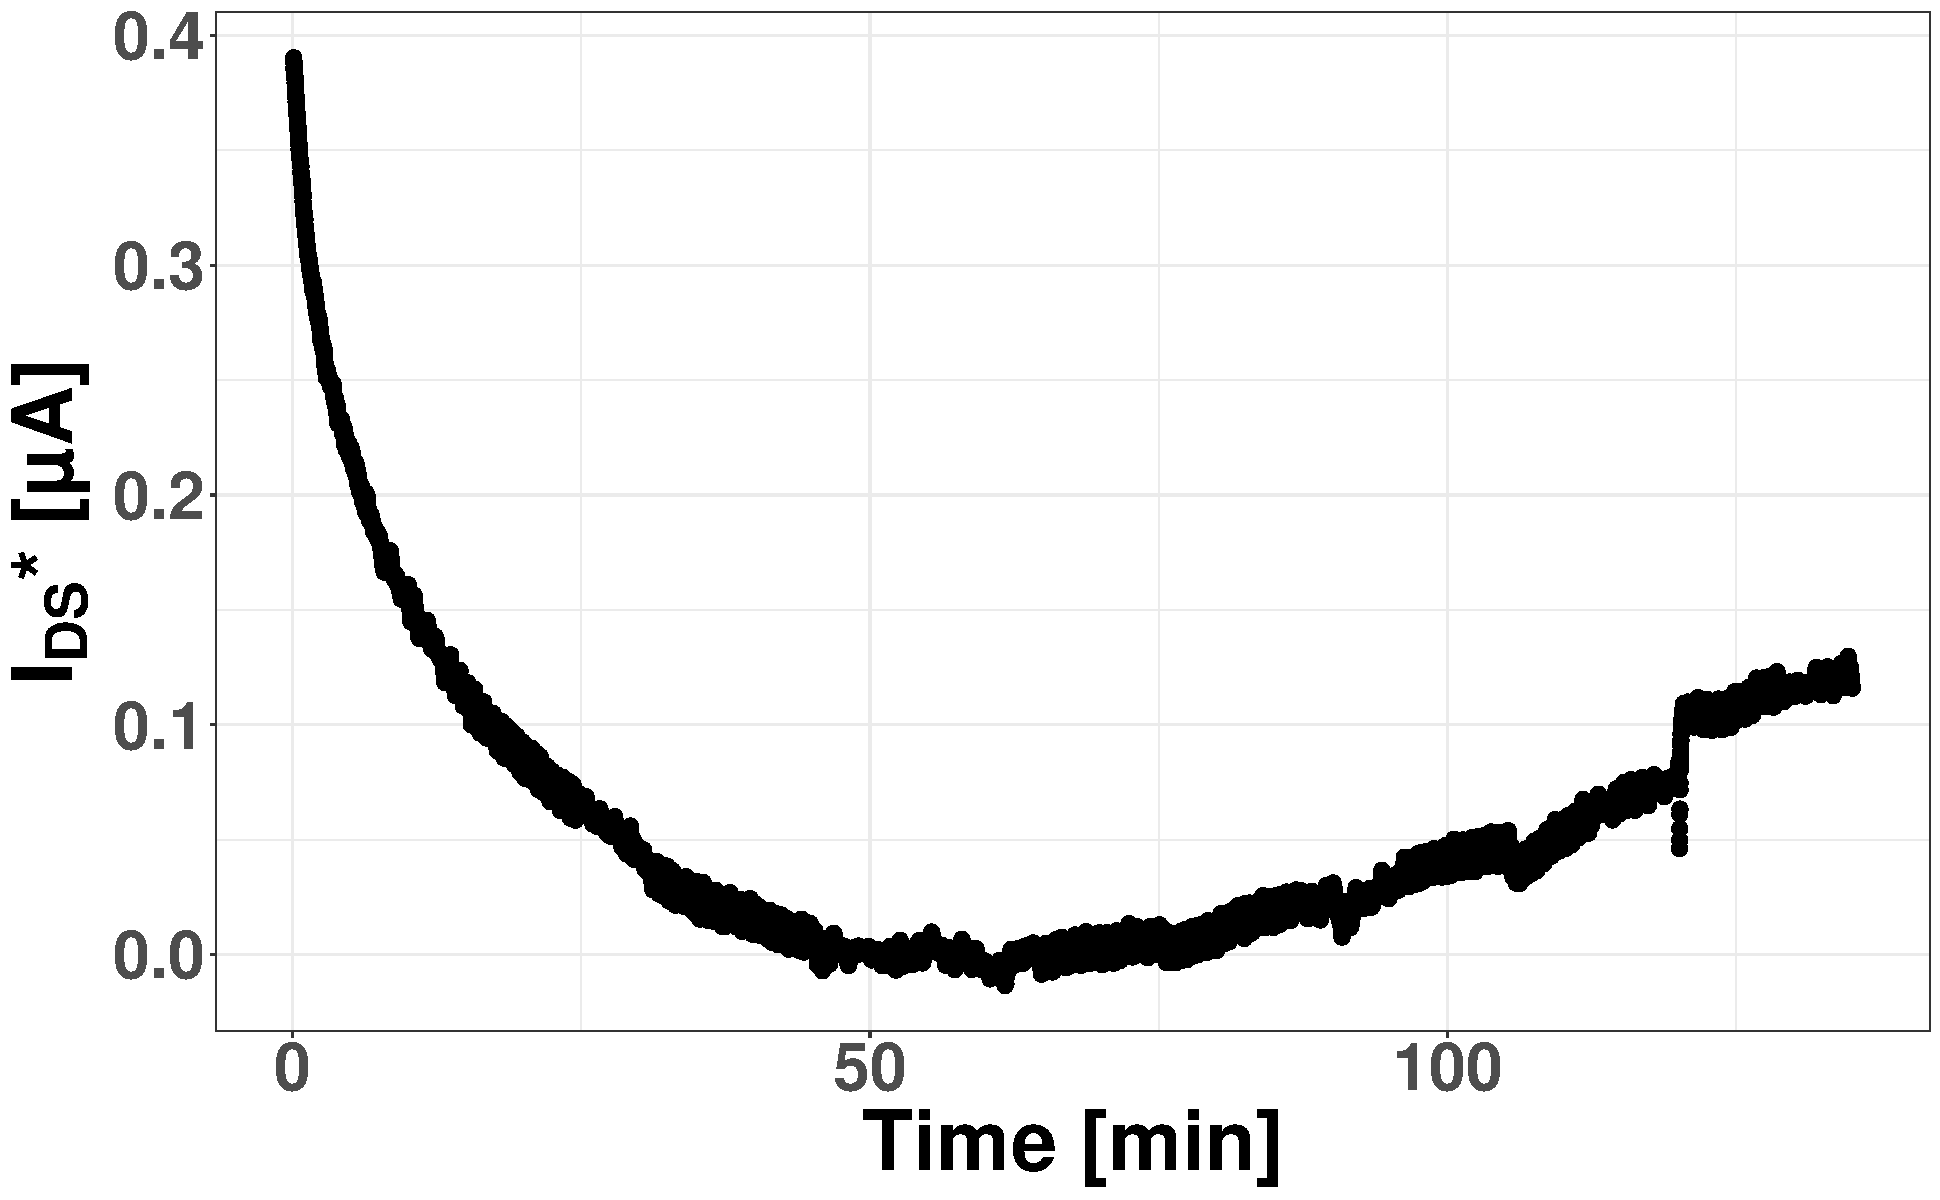
\includegraphics[width = 0.4\textwidth]{figures/chapter4/histamine/correctedPlot-chronoamperometry.pdf}
    \quad
    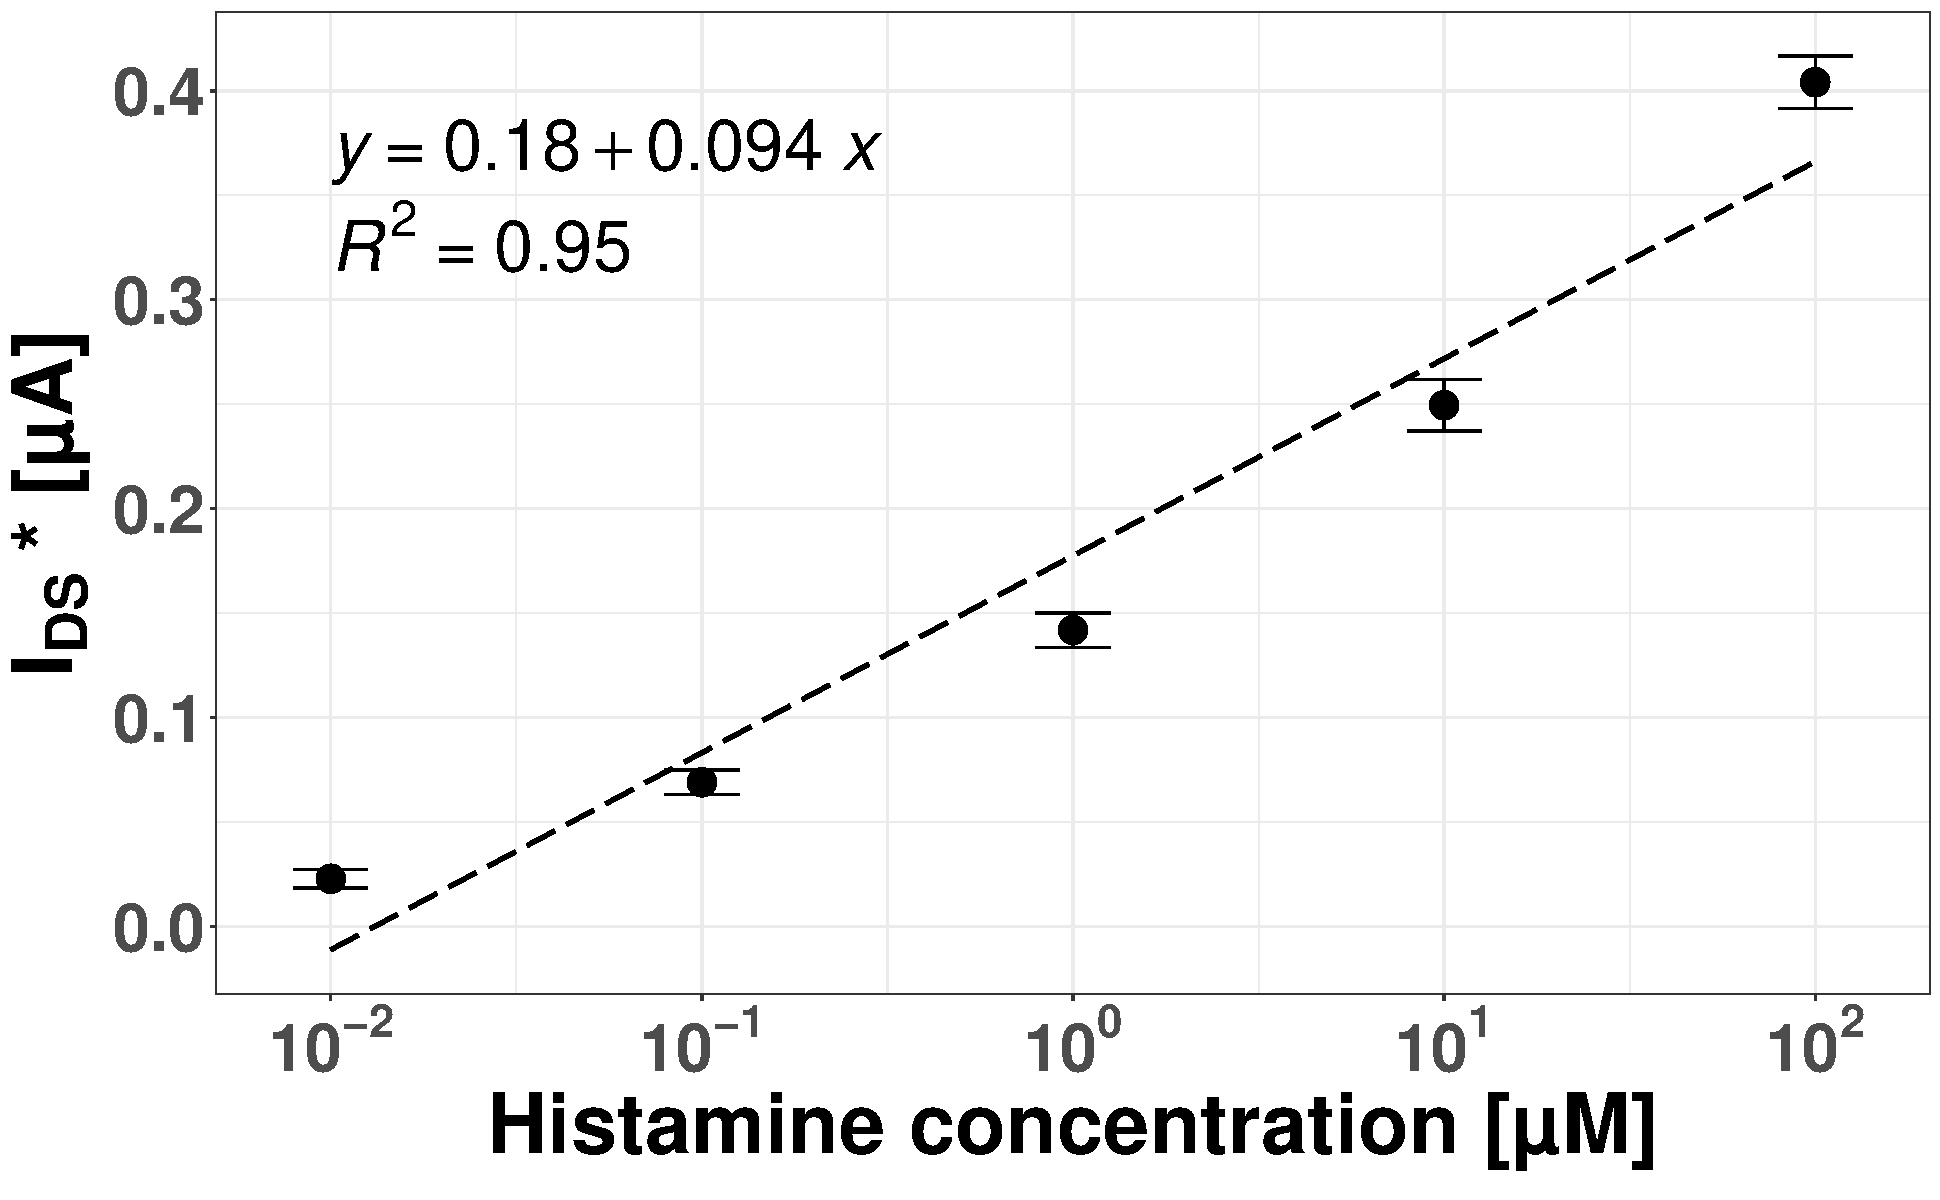
\includegraphics[width = 0.4\textwidth]{figures/chapter4/histamine/calibrationPlot-chronoamperometry.pdf}
    \caption{}
    \label{fig:HisChrono}
\end{figure}

